\chapter{\IfLanguageName{dutch}{Corpus}{Corpus}}
\label{ch:corpus}

\section{\IfLanguageName{dutch}{Proof of concept}{Proof of concept}}
\label{ch:proof-of-concept}

Voor de proof of concept is de Arduino gekozen omdat dit een microcontroller is. Microcontrollers zijn zuiniger qua stroomgebruik ten opzichte van een 'computer' (Raspberry Pi). Hierdoor heeft de Arduino een langere batterijduur. Naast het verbruik is het eveneens goedkoper (zie hoofdstuk \ref{ch:stand-van-zaken}).

\subsection{\IfLanguageName{dutch}{Opstelling proof of concept}{Setup proof of concept}}
De \textbf{uitgewerkte proof of concept} (zie figuur: \ref{fig:opstelling_arduino}) bestaat uit:
\begin{itemize}
	\item Arduino MKR GSM 1400 Cellular Kit (80.35 euro);
	\item Arduino MKR GPS Shield (41.75 euro);
	\item Lithium Ion Polymeer Accu - 3.7V 2500mAh (25.90 euro).
\end{itemize}
De totale kost van de proof of concept komt neer op \textbf{148.00 euro}. Naast de lage kost heeft de proof of concept het voordeel dat hij volledig zelf geconfigureerd kan worden. In functie van het onderzoek werd een eigen script ontwikkeld. De configuratie is gebeurd in de editor van Arduino zelf. Het script is in staat om de volgende functies uit te voeren:
\begin{itemize}
	\item De locatie bepalen aan de hand van GPS;
	\item De locatie bepalen aan de hand van GPRS;
	\item De locatie doorsturen naar een REST API aan de hand van een POST-request (JSON).
\end{itemize}
Het script is innovatief en staat open source op \underline{\href{https://github.com/IndyVC/bap-arduino}{een github repository}}. In het script werd gebruik gemaakt van verschillende libraries om het traceren mogelijk te maken.
Er werd gebruik gemaakt van:
\begin{itemize}
	\item \href{https://github.com/arduino-libraries/ArduinoHttpClient}{ArduinoHttpClient}: voor het versturen van data aan de hand van POST requests;
	\item \href{https://github.com/arduino-libraries/MKRGSM}{MKRGSM}: voor het gebruik van mobiele data;
	\item \href{https://github.com/bblanchon/ArduinoJson}{ArduinoJson}: het mogelijk maken om makkelijk een JSON body op te vullen;
	\item \href{https://github.com/arduino-libraries/Arduino_MKRGPS}{ArduinoMKRGPS}: voor het bepalen van de locatie via GPS.
\end{itemize}
De proof of concept maakt gebruik van een simkaart (zie figuur: \ref{fig:simkaart}) om online data te kunnen versturen. 
\begin{figure}
	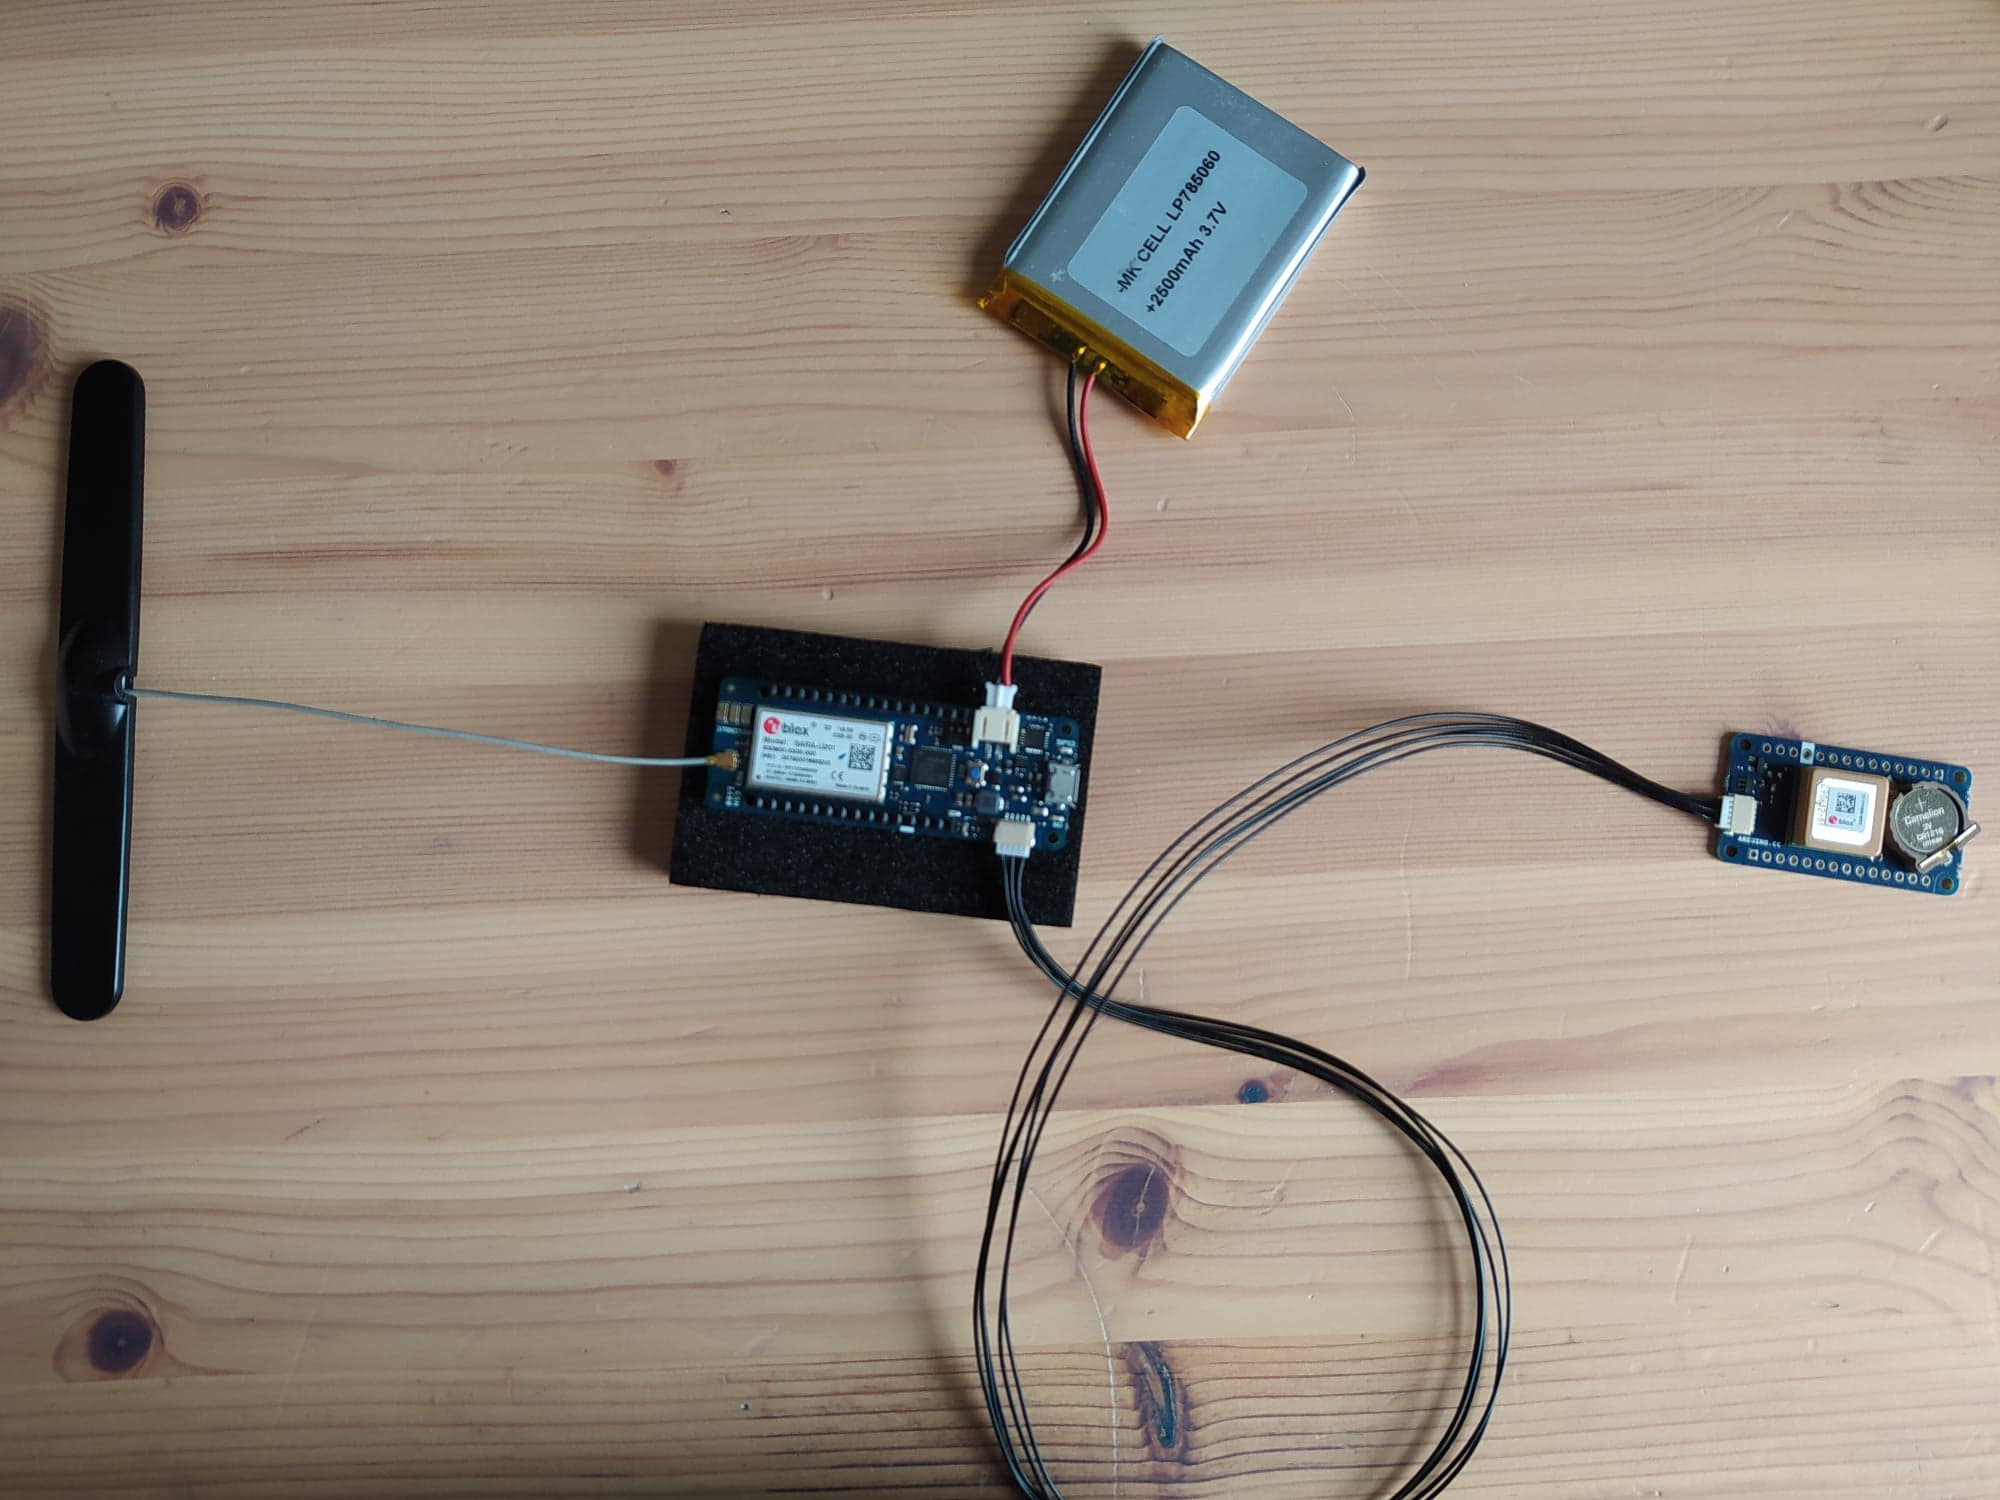
\includegraphics[width=\textwidth,height=\textheight,keepaspectratio]{opstelling_arduino.jpg}
	\caption{opstelling proof of concept}
	\label{fig:opstelling_arduino}
\end{figure}
\begin{figure}
	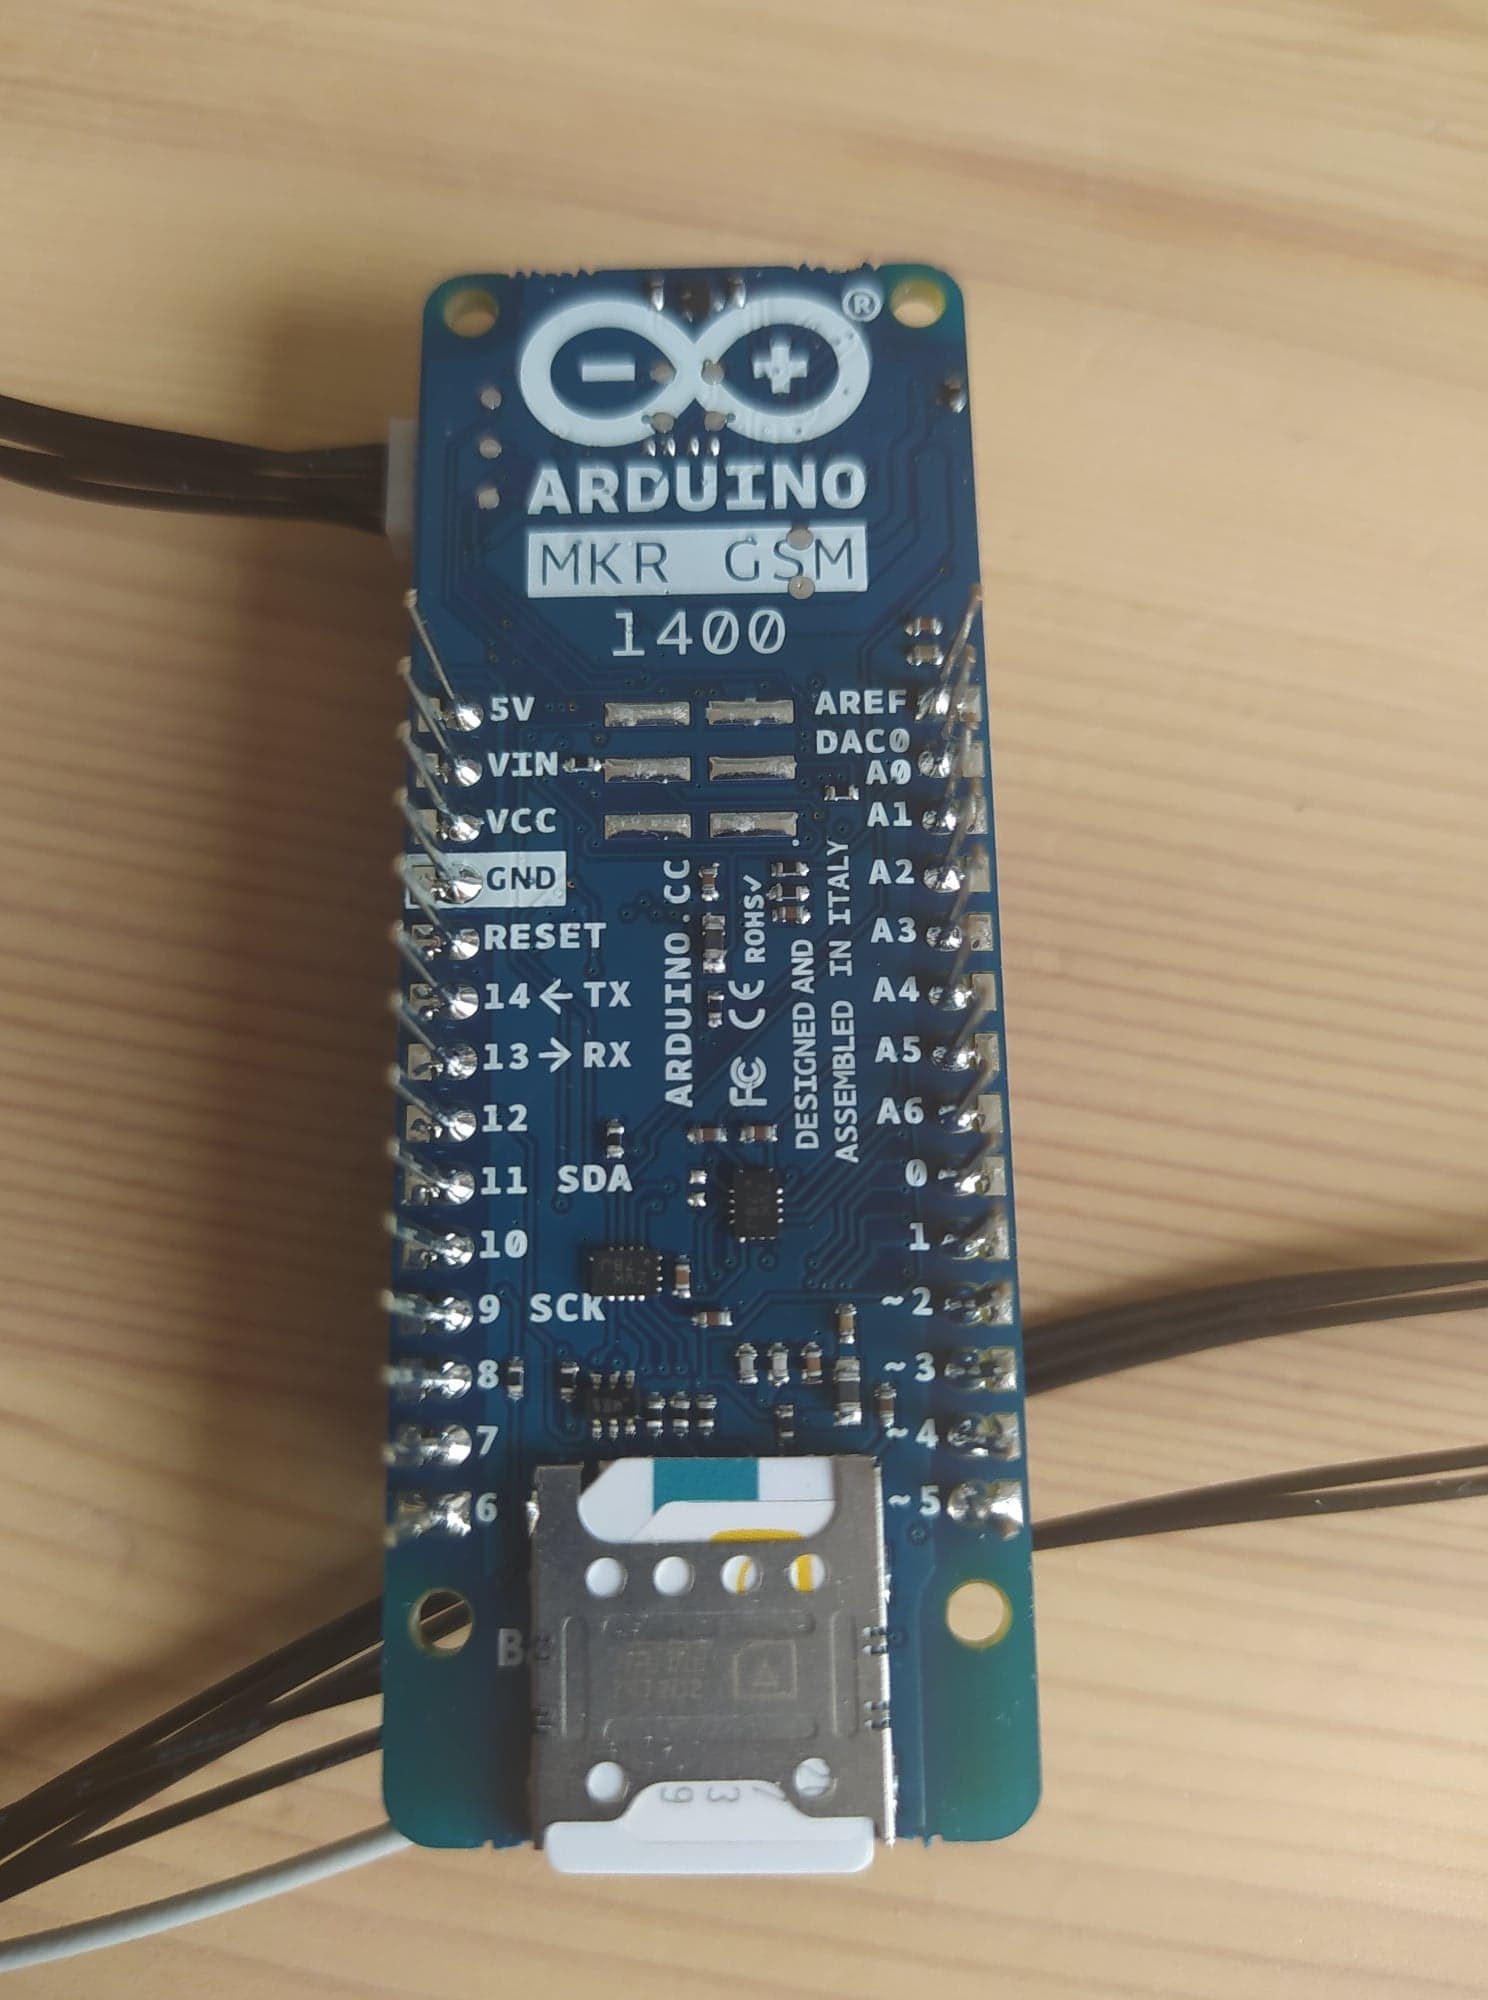
\includegraphics[width=\textwidth,height=\textheight,keepaspectratio]{simkaart.jpg}
	\caption[Achterkant MKR 1400 gsm module]{Achterkant van de MKR 1400 gsm module waar de simkaart wordt geplaatst}
	\label{fig:simkaart}
\end{figure}
\pagebreak
\subsection{\IfLanguageName{dutch}{Waterdichte casing}{Waterproof casing}}
Het maken van een waterdichte behuizing is niet eenvoudig. In de ontwikkelingsfase werden twee modellen uitgeprint en getest. Daaruit bleek dat beide modellen niet waterdicht waren. Dit komt doordat de gebruikte 3D-printer (Anycubic Predator) niet nauwkeurig genoeg is om waterdichtheid te garanderen. Bovendien beschikt het gebruikte materiaal (PLA) niet over de juiste eigenschappen. Door de coronapandemie is het praktisch niet mogelijk om een nieuwe behuizing te ontwikkelen die wel waterdicht is. Daarom is er noodgedwongen gebruik gemaakt van een aftakdoos. Deze doos is volledig waterdicht en beschikt over een grote binnenruimte. Dit wilt zeggen dat er schokdemping toegevoegd kan worden zodat de proof of concept niet beschadigd wordt. De prijs is 18,14 euro.
\begin{figure}
	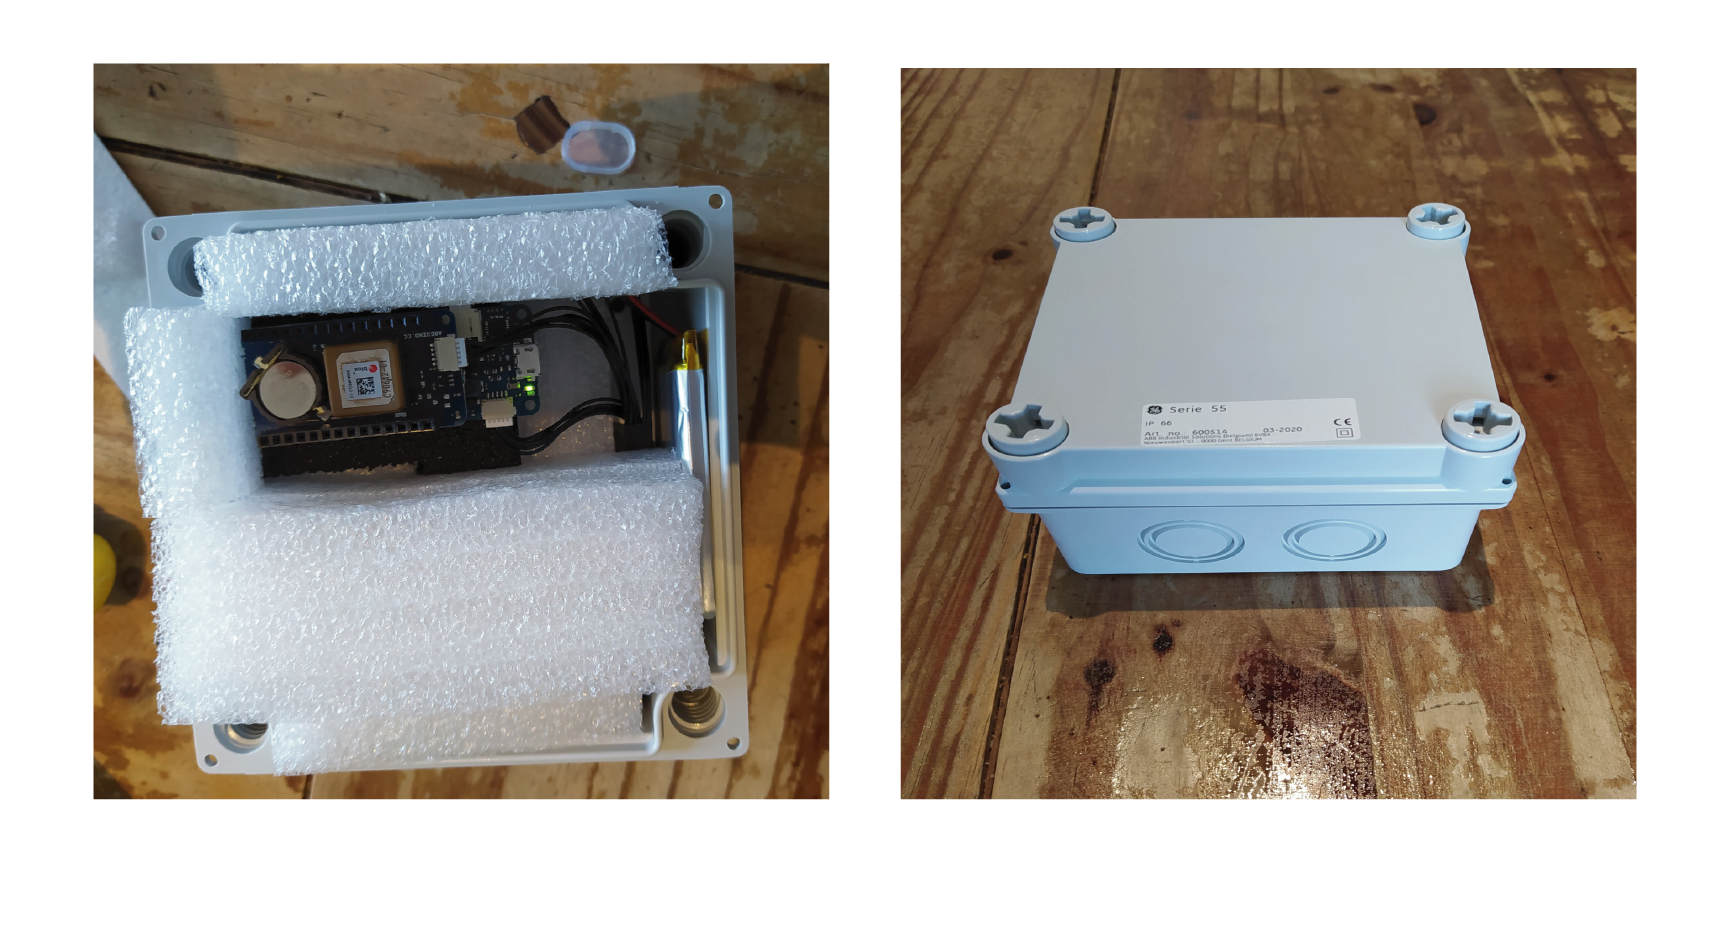
\includegraphics[width=\textwidth,height=\textheight,keepaspectratio]{aftakdoos.jpg}
	\caption{Waterdichte behuizing}
	\label{fig:case}
\end{figure}
\section{\IfLanguageName{dutch}{Backend}{Backend}}
\label{ch:backend}

\subsection{\IfLanguageName{dutch}{Ontwikkeling}{Development}}
Voor backend is er gebruik gemaakt van \href{https://mongoosejs.com/}{Mongoose}. De gehele infrastructuur is gebaseerd op de MEVN-stack.
Deze stack staat voor:
\begin{itemize}
	\item Mongoose
	\item Express
	\item Vue
	\item Node.JS
\end{itemize}
Mongoose maakt gebruik van \href{https://www.mongodb.com/cloud/atlas}{MongoDB Atlas}. De backend, geschreven in Javascript, is open source en staat online op \underline{\href{https://github.com/IndyVC/bap-backend}{een github repository}}.
\newline
De functie van de backend is om locaties van de proof of concept te ontvangen. Deze locaties worden opgeslagen in een NO-SQL database. De database slaagt per locatie de volgende gegevens op:
\begin{itemize}
	\item Longitude
	\item Latitude
	\item Altitude
	\item Snelheid (in km/h)
	\item Aantal satellieten
	\item Method (locatie bepaalt via GPS of GPRS)
\end{itemize}
De methodiek hangt af van de beschikbaarheid van het signaal. Indien er geen GPS-signaal gevonden kan worden, schakelt de proof of concept automatisch over op GPRS. Maar GPS blijft wel de eerste keuze omdat dit accurater is dan GPRS. Indien de locatie bepaald is via GPRS, heeft men geen informatie over de snelheid en het aantal satellieten. GPRS-data worden immers bepaald op basis van gsm-masten (zie hoofdstuk \ref{ch:stand-van-zaken}).

\subsection{\IfLanguageName{dutch}{Deployment}{Deployment}}
Naast de code staat ook het programma online. De backend kan \href{https://indy-bap-backend.herokuapp.com/api/locations}{\underline{hier}} bekeken worden. Voor de deployment is er gebruik gemaakt van \href{www.heroku.com}{Heroku}. Doordat het programma online draait, kan de \href{https://indy-bap-frontend.netlify.com/}{webapplicatie} deze data ophalen en weergeven.
\newline
De backend maakt gebruik van een gratis hosting plan, dit kan nadelig zijn. Het programma kan na 30 minuten inactiviteit in slaapstand gaan. Dat wil zeggen dat de webapplicatie twee keer moet opgeladen worden. De eerste keer dient om de backend terug te activeren, de tweede keer om effectief te gebruiken.
\pagebreak
\section{\IfLanguageName{dutch}{Frontend}{Frontend}}
\label{ch:frontend}

\subsection{\IfLanguageName{dutch}{Ontwikkeling}{Development}}
Zoals reeds verteld is er gebruik gemaakt van de MEVN-stack. Dit wil zeggen dat de webapplicatie ontwikkeld is in Vue, een nieuwer javascript-framework. De code van deze webapplicatie is open source en staat online op \underline{\href{https://github.com/IndyVC/bap-frontend}{een github repository}}.
\newline
Voor de webapplicatie (zie figuur: \ref{fig:webapplicatie}) is er gebruik gemaakt van 'Google Maps'. Google Maps is een populaire online kaartendienst waarmee geografische locaties kunnen opgezocht worden waardoor dezelfde layout een vorm van betrouwbaarheid en herkenbaarheid geeft voor de aankoper van het toestel. Dit bevordert de gebruiksvriendelijkheid van de webapplicatie. Naast het tracken zelf, geeft het ook extra informatie weer, zoals welke methode gebruikt wordt, hoe snel de GPS-tracker zich voortbeweegt en hoe betrouwbaar de coördinaten zijn (aantal satellieten). De gebruiker kan de geschiedenis van de locaties wissen via een knop.
\newline
Voor de implementatie van Google Maps is er gebruik gemaakt van een open source en gratis te gebruiken library, namelijk \href{https://www.npmjs.com/package/vue2-google-maps}{vue2-google-maps}.
\begin{figure}
	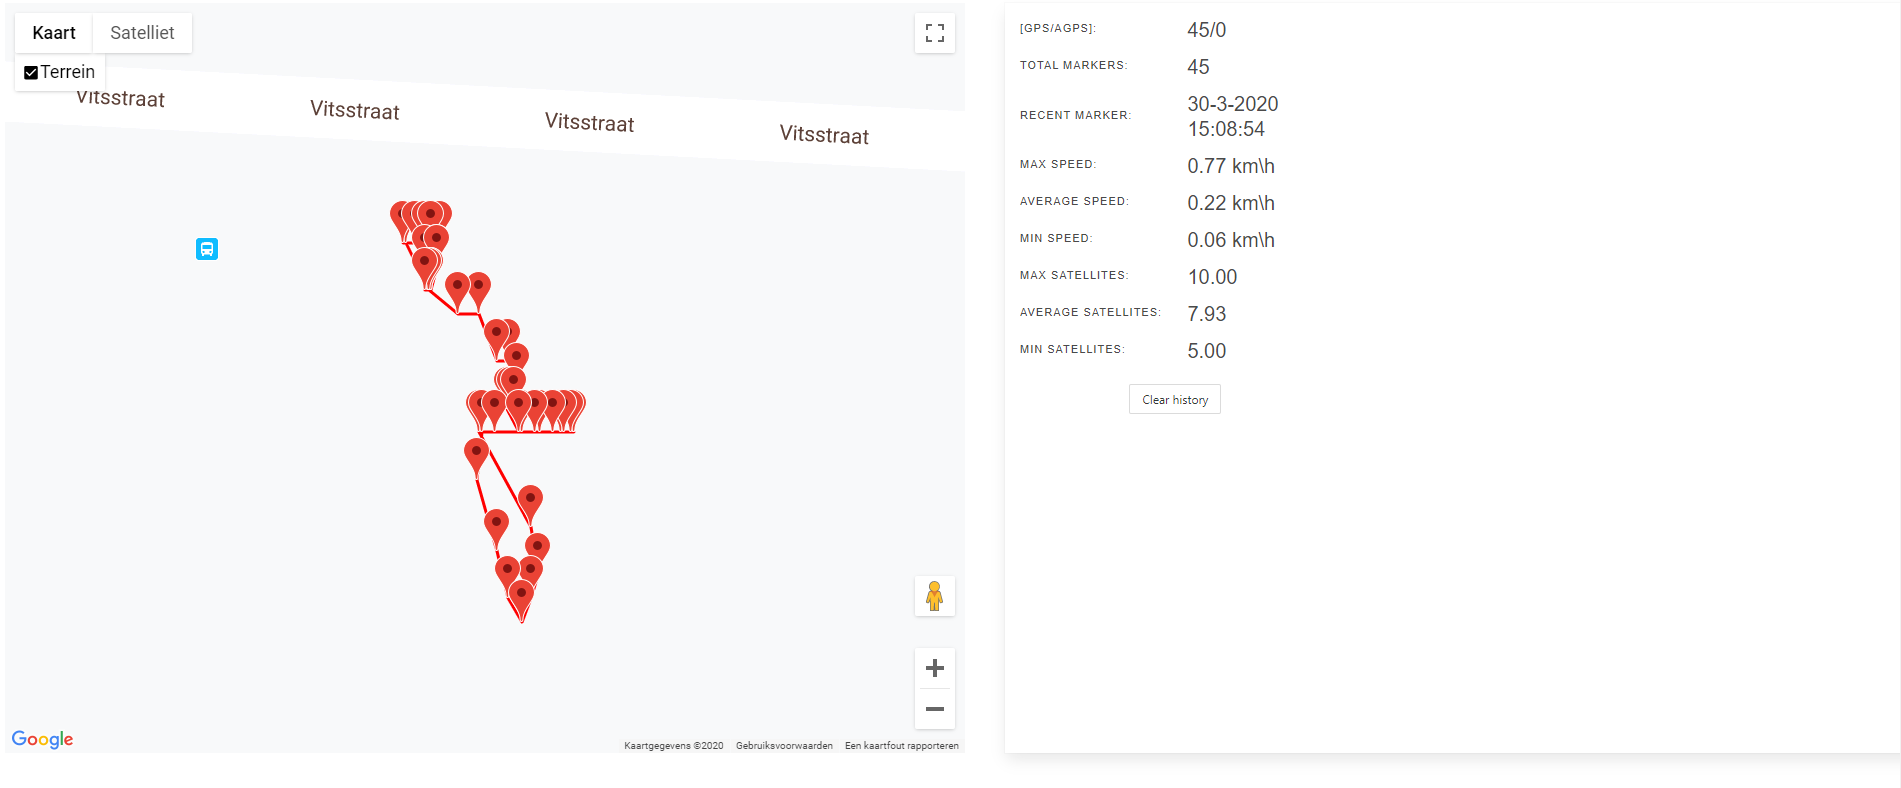
\includegraphics[width=\textwidth,height=\textheight,keepaspectratio]{webapplicatie.png}
	\caption{Zelf ontwikkelde webapplicatie}
	\label{fig:webapplicatie}
\end{figure}

\subsection{\IfLanguageName{dutch}{Deployment}{Deployment}}
Om de website online te zetten is er gebruik gemaakt van Netlify. \href{https://www.netlify.com/}{Netlify} is een hosting bedrijf dat een gratis plan aanbiedt. De webapplicatie staat \href{https://indy-bap-frontend.netlify.com/}{\underline{hier}} online.

\section{\IfLanguageName{dutch}{Mobiele applicatie}{Mobile application}}
\label{ch:mobileapp}
Om de vergelijking te kunnen maken tussen de GPS in een gsm en de proof of concept, is er een mobiele applicatie ontwikkeld (zie figuur: \ref{fig:mobileapp}). Deze mobiele applicatie herberekent de locatie met een interval van drie seconden, waarna ze dan wordt doorgestuurd naar de backend. (sectie \ref{ch:backend}). De mobiele applicatie is ontwikkeld in \href{https://www.nativescript.org/}{NativeScript}. NativeScript is een open source framework dat gebruikt kan worden om native mobiele applicaties te maken voor Android en iOS. Om NativeScript te gebruiken kan er gekozen worden uit vier opties om de app te ontwikkelen:
\begin{itemize}
	\item Angular
	\item Vue
	\item Javascript
	\item Typescript
\end{itemize}
Voor de mobiele applicatie is er gebruik gemaakt van Vue. De code van de mobiele applicatie is open source en staat online op \underline{\href{https://github.com/IndyVC/bap-gsmtracker}{een github repository}}. 
\begin{figure}
	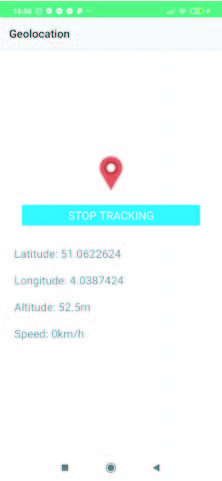
\includegraphics[width=\textwidth,height=\textheight,keepaspectratio]{mobile_app.jpg}
	\caption{Zelf ontwikkelde mobiele applicatie}
	\label{fig:mobileapp}
\end{figure}